\newif\ifadvisor\advisorfalse
\newcommand{\advisor}[2]{\ifadvisor#1\else#2\fi}
\newcommand{\brazilword}[1]{#1}

\PassOptionsToPackage{main=brazil,english}{babel}

\documentclass[
brazilian,brazil,
12pt,
a4paper,
oneside,
chapter=TITLE,
section=TITLE,
]{setup/ufscthesisx}

\addbibresource{references.bib}

\autor{Gabriel Salmoria \\ Lucas de Souza Vieira}
\titulo{IBE Mail: Criptografia Baseada em Identidade com o Esquema de Boneh-Franklin}
\tipotrabalho{Relatório Final}
\local{Florianópolis -- SC}
\ano{2026}
\data{Julho de 2026}
\instituicaosigla{UFSC}
\instituicao{Universidade Federal de Santa Catarina}
\area{Segurança em Computação}
\centro{INE -- Departamento de Informática e Estatística, CTC -- Centro Tecnológico}
\campus{Campus Reitor João David Ferreira Lima}
\orientador[Professores]{Jean Martina e Thaís Bardini Idalino}

\hypersetup{
    pdfcreator={LaTeX with abnTeX2 for UFSC},
    pdftitle={\imprimirtitulo},
    pdfauthor={Gabriel Salmoria e Lucas de Souza Vieira},
}

%----------------------------------------------------------------------------------------
%   Thesis Tweaks and Utilities
%----------------------------------------------------------------------------------------
\makeatletter

% Load additional babel languages after the class has already loaded babel.
% Using \babelprovide instead of package options for compatibility with babel >= 3.x.
\babelprovide{spanish}
\babelprovide{french}

\usepackage{lipsum}
\usepackage{algorithm}
\usepackage{algpseudocode}


% Uncomment this if you are debugging pages' badness Underfull & Overflow
% https://tex.stackexchange.com/questions/115908/geometry-showframe-landscape
% https://tex.stackexchange.com/questions/387077/what-is-the-difference-between-usepackageshowframe-and-usepackageshowframe
% https://tex.stackexchange.com/questions/387257/how-to-do-the-memoir-headings-fix-but-not-have-my-text-going-over-the-page-botto
% https://tex.stackexchange.com/questions/14508/print-page-margins-of-a-document
% \usepackage[showframe,pass]{geometry}

% To use the font Times New Roman, instead of the default LaTeX font
% more up-to-date than '\usepackage{mathptmx}'
% \usepackage{newtxtext}
% \usepackage{newtxmath}

% https://tex.stackexchange.com/questions/182569/how-to-manually-set-where-a-word-is-split
\hyphenation{Ge-la-im}
\hyphenation{Cis-la-ghi}

% Add missing translations for Portuguese
% https://tex.stackexchange.com/questions/8564/what-is-the-right-way-to-redefine-macros-defined-by-babel
\@ifpackageloaded{babel}{\@ifpackagewith{babel}{brazil}{\addto\captionsbrazil{%
  \renewcommand{\mytextpreliminarylistname}{Breve Sumário}
}}{}}{}
\@ifundefined{advisor}{\newcommand{\advisor}[2]{#1}}{}

% Selects a sans serif font family
% \renewcommand{\sfdefault}{cmss}

% Selects a monospaced (“typewriter”) font family
% \renewcommand{\ttdefault}{cmtt}

% Use OpenType Latin Modern fonts in LuaLaTeX for full Unicode support.
% This gives the identical look as default LaTeX (Computer Modern) but with Unicode.
\usepackage{iftex}
\ifLuaTeX
  \usepackage{fontspec}
  \setmainfont{Latin Modern Roman}
  \setsansfont{Latin Modern Sans}
  \setmonofont{Latin Modern Mono}
\fi

% Spacing between lines and paragraphs
% https://tex.stackexchange.com/questions/70212/ifpackageloaded-question
\@ifclassloaded{memoir}
{
  % New custom chapter style VZ14, see other chapters styles in:
  % http://repositorios.cpai.unb.br/ctan/info/latex-samples/MemoirChapStyles/MemoirChapStyles.pdf
  \newcommand\thickhrulefill{\leavevmode \leaders \hrule height 1ex \hfill \kern \z@}
  \makechapterstyle{VZ14} { %
    % \thispagestyle{empty}
    \setlength\beforechapskip{50pt}
    \setlength\midchapskip{20pt}
    \setlength\afterchapskip{20pt}
    \renewcommand\chapternamenum{}
    \renewcommand\printchaptername{}
    \renewcommand\chapnamefont{\Huge\scshape}
    \renewcommand\printchapternum {%
      \chapnamefont\null\thickhrulefill\quad
      \@chapapp\space\thechapter\quad\thickhrulefill
    }
    \renewcommand\printchapternonum {%
      \par\thickhrulefill\par\vskip\midchapskip
      \hrule\vskip\midchapskip
    }
    \renewcommand\chaptitlefont{\huge\scshape\centering}
    \renewcommand\afterchapternum {%
      \par\nobreak\vskip\midchapskip\hrule\vskip\midchapskip
    }
    \renewcommand\afterchaptertitle {%
      \par\vskip\midchapskip\hrule\nobreak\vskip\afterchapskip
    }
  }

  % Apply the style `VZ14` just created
  % \chapterstyle{VZ14}

  % http://mirrors.ibiblio.org/CTAN/macros/latex/contrib/memoir/memman.pdf
  \setlength\beforechapskip{0pt}
  \setlength\midchapskip{15pt}
  \setlength\afterchapskip{15pt}

  % Memoir: Warnings “The material used in the headers is too large” w/ accented titles
  % https://tex.stackexchange.com/questions/387293/how-to-change-the-page-layout-with-memoir
  \setheadfoot{30.0pt}{\footskip}
  \checkandfixthelayout
}{}

% Controlling the spacing between one paragraph and another
% Default value for UFSC 0.0cm
\setlength{\parskip}{\advisor{0.0cm}{0.2cm}}

% Paragraph size is given by
% Default value for UFSC 1.5cm
% \setlength{\parindent}{1.3cm}

% https://tex.stackexchange.com/questions/148647/how-to-remove-space-before-enumerate
% https://tex.stackexchange.com/questions/433543/behaviour-of-enumitem-setlist
\advisor{}{
    \setlist*[enumerate]{label=\arabic*,}
    \setlist*[enumerateoptional]{label=\arabic*,}

    % https://tex.stackexchange.com/questions/24454/space-after-float-with-h
    % https://tex.stackexchange.com/questions/23313/how-can-i-reduce-padding-after-figure
    \AtBeginEnvironment{figure}{
      \setlength{\intextsep}{5pt} % Vertical space above & below [h] floats
      % \setlength{\textfloatsep}{10pt} % Vertical space below (above) [t] ([b]) floats
      % \setlength{\abovecaptionskip}{10pt}
      % \setlength{\belowcaptionskip}{5pt}
    }

    % Patch the `abntex2` citacao environment removing the extra space from its top
    % https://tex.stackexchange.com/questions/300340/topsep-itemsep-partopsep-and-parsep-what-does-each-of-them-mean-and-wha
    \xpatchcmd{\citacao}
    {\list{}}
    {\list{}{\topsep=0pt}}
    {}
    {\FAILEDPATCHINGCITACAO}
}


% Color settings across the document
\@ifpackageloaded{xcolor}
{
  % RGB colors in absolute values from 0 to 255 by using `RGB` tag
  \definecolor{darkblue}{RGB}{26,13,178}

  % Colors names definitions as RGB colors in percentage notation by using `rgb` tag
  \definecolor{mygreen}{rgb}{0,0.6,0}
  \definecolor{mygray}{rgb}{0.5,0.5,0.5}
  \definecolor{mymauve}{rgb}{0.58,0,0.82}
  \definecolor{figcolor}{rgb}{1,0.4,0}
  \definecolor{tabcolor}{rgb}{1,0.4,0}
  \definecolor{eqncolor}{rgb}{1,0.4,0}
  \definecolor{linkcolor}{rgb}{1,0.4,0}
  \definecolor{citecolor}{rgb}{1,0.4,0}
  \definecolor{seccolor}{rgb}{0,0,1}
  \definecolor{abscolor}{rgb}{0,0,1}
  \definecolor{titlecolor}{rgb}{0,0,1}
  \definecolor{biocolor}{rgb}{0,0,1}
  \definecolor{blue}{RGB}{41,5,195}

  % PDF Hyperlinks settings
  \@ifpackageloaded{hyperref}
  {
    \hypersetup
    {
      hidelinks,
      bookmarksdepth=4,
      pdfencoding=auto,
      psdextra,
    }
  }
}{}


% Filtering and Mapping Bibliographies
% \DeclareFieldFormat{url}{Disponível~em:\addspace\url{#1}}

% https://tex.stackexchange.com/questions/517526/how-to-make-biblatex-url-links-generated-with-brackets-around-it-url-correctly
\DeclareFieldFormat{url}{\bibstring{urlfrom}\addcolon\space\textless\url{#1}\textgreater}
\DefineBibliographyStrings{brazil}{urlfrom = {Disponível em}}
\DefineBibliographyStrings{english}{urlfrom = {Available from}}

% https://tex.stackexchange.com/questions/391695/is-possible-to-remove-the-link-color-of-the-comma-on-the-citation-link
% \DeclareFieldFormat{citehyperref}{#1}

% % https://tex.stackexchange.com/questions/203764/reduce-font-size-of-bibliography-overfull-bibliography
% \newcommand{\bibliographyfontsize}{\fontsize{10.0pt}{10.5pt}\selectfont}
% \renewcommand*{\bibfont}{\bibliographyfontsize}

% Uncomment this to insert the abstract into your bibliography entries when the abstract is available
% https://tex.stackexchange.com/questions/398666/how-to-correctly-insert-and-justify-abstract
\ifadvisor
\else
  \DeclareFieldFormat{abstract}%
  {%
    \par\justifying
    \begin{adjustwidth}{1cm}{}
      \textbf{\bibsentence\bibstring{abstract}:} #1
    \end{adjustwidth}
  }
  \renewbibmacro*{finentry}%
  {%
    \iffieldundef{abstract}
    {\finentry}
    {\finentrypunct
      \printfield{abstract}%
      \renewcommand*{\finentrypunct}{}%
      \finentry
    }
  }

  % Backref package settings, pages with citations in bibliography
  \newcommand{\biblatexcitedntimes}{\autocap{c}ited \arabic{citecounter} times}
  \newcommand{\biblatexcitedonetime}{\autocap{c}ited one time}
  \newcommand{\biblatexcitednotimes}{\autocap{n}o citation in the text}

  \@ifpackageloaded{babel}{\@ifpackagewith{babel}{brazil}{\addto\captionsbrazil{%
    \renewcommand{\biblatexcitedntimes}{\autocap{c}itado \arabic{citecounter} vezes}
    \renewcommand{\biblatexcitedonetime}{\autocap{c}itado uma vez}
    \renewcommand{\biblatexcitednotimes}{\autocap{n}enhuma citação no texto}
  }}{}}{}
  \@ifpackageloaded{biblatex}
  {%
    % https://tex.stackexchange.com/questions/483707/how-to-detect-whether-the-option-citecounter-was-enabled-on-biblatex
    \ifx\blx@citecounter\relax
      \message{Is citecounter defined? NO!^^J}
    \else
      \message{Is citecounter defined? YES!^^J}
      \ifbacktracker
        \message{Is backtracker defined? YES!^^J}
        \renewbibmacro*{pageref}
        {%
          % https://tex.stackexchange.com/questions/516054/how-to-use-a-dot-to-separate-my-new-bibliography-entry
          \renewcommand*{\bibpagerefpunct}{\addperiod\space}%
          \iflistundef{pageref}%
          {\printtext{\biblatexcitednotimes}}
          {%
            \printtext
            {%
              \ifnumgreater{\value{citecounter}}{1}
                {\biblatexcitedntimes}
                {\biblatexcitedonetime}%
            }%
            \setunit{\addspace}%
            \ifnumgreater{\value{pageref}}{1}
              {\bibstring{backrefpages}\ppspace}
              {\bibstring{backrefpage}\ppspace}%
            \printlist[pageref][-\value{listtotal}]{pageref}%
          }%
        }

        \DefineBibliographyStrings{brazil}
        {
          backrefpage  = {na página},
          backrefpages = {nas páginas},
        }

        \DefineBibliographyStrings{english}
        {
          backrefpage  = {on page},
          backrefpages = {on pages},
        }
      \else
        \message{Is backtracker defined? NO!^^J}
      \fi
    \fi
  }{}
\fi


% https://tex.stackexchange.com/questions/516056/why-an-empty-or-not-biblatex-declaresourcemap-is-removing-my-bibliography-acces
% https://github.com/abntex/biblatex-abnt/pull/56/files
\DeclareStyleSourcemap{%% >>>2
  % This maps some fields used in abntex2cite to biblatex fields.
  \maps[datatype=bibtex]{%
    \map{%
      \step[fieldsource=conference-number,fieldtarget=number]%
      \step[fieldsource=conference-year,fieldtarget=eventdate]%
      \step[fieldsource=conference-location,fieldtarget=venue]%
      \step[fieldsource=conference-number,fieldtarget=number]%
      \step[fieldsource=org-short,fieldtarget=shortauthor]%
      \step[fieldsource=urlaccessdate,fieldtarget=urldate]%
      \step[fieldsource=year-presented,fieldtarget=eventyear]%
      \step[fieldsource=furtherresp,fieldtarget=titleaddon]%
      \step[typesource=journalpart,typetarget=supperiodical]%
    }%
    \map[overwrite=false]{%
      \step[fieldsource=reprinted-from, final]%
      \step[fieldset=related, origfieldval]%
    }%
    \map[overwrite=false]{%
      \step[fieldsource=reprinted-text, final]%
      \step[fieldset=relatedtype, fieldvalue={reprintfrom}]%
    }%
    \map{%
      \pertype{patent}% Use the organization as sourcekey for patents
      \step[fieldsource=organization, final]%
      \step[fieldset=sortkey, origfieldval]%
    }%
    \map[overwrite=false]{%
      \pertype{thesis}%
      \pertype{phdthesis}%
      \pertype{mastersthesis}%
      \pertype{monography}%
      \step[fieldset=bookpagination, fieldvalue={sheet}]%
    }%
    % remove fields that are always useless
    \map{
      % \step[fieldset=abstract, null]
      \step[fieldset=pagetotal, null]
    }
    % % remove URLs for types that are primarily printed
    % \map{
    %   \pernottype{software}
    %   \pernottype{online}
    %   \pernottype{report}
    %   \pernottype{techreport}
    %   \pernottype{standard}
    %   \pernottype{manual}
    %   \pernottype{misc}
    %   \step[fieldset=url, null]
    %   \step[fieldset=urldate, null]
    % }
    \map{
      \pertype{inproceedings}
      % remove mostly redundant conference information
      \step[fieldset=venue, null]
      \step[fieldset=eventdate, null]
      \step[fieldset=eventtitle, null]
      % do not show ISBN for proceedings
      \step[fieldset=isbn, null]
      % Citavi bug
      \step[fieldset=volume, null]
    }
  }%
}% <<<2


% https://tex.stackexchange.com/questions/14314/changing-the-font-of-the-numbers-in-the-toc-in-the-memoir-class
\renewcommand{\cftpartfont}{\ABNTEXpartfont\color{black}}
\renewcommand{\cftpartpagefont}{\ABNTEXpartfont\color{black}}

\renewcommand{\cftchapterfont}{\ABNTEXchapterfont\color{black}}
\renewcommand{\cftchapterpagefont}{\ABNTEXchapterfont\color{black}}

\renewcommand{\cftsectionfont}{\ABNTEXsectionfont\color{black}}
\renewcommand{\cftsectionpagefont}{\ABNTEXsectionfont\color{black}}

\renewcommand{\cftsubsectionfont}{\ABNTEXsectionfont\color{black}}
\renewcommand{\cftsubsectionpagefont}{\ABNTEXsectionfont\color{black}}

\renewcommand{\cftsubsubsectionfont}{\ABNTEXsubsubsectionfont\color{black}}
\renewcommand{\cftsubsubsectionpagefont}{\ABNTEXsubsubsectionfont\color{black}}

\renewcommand{\cftparagraphfont}{\ABNTEXsubsubsubsectionfont\color{black}}
\renewcommand{\cftparagraphpagefont}{\ABNTEXsubsubsubsectionfont\color{black}}

% Memoir has another mechanism for the job: \cftsetindents{‹kind›}{indent}{numwidth}. Here kind is
% chapter, section, or whatever; the indent specifies the ‘margin’ before the entry starts; and the
% width is of the box into which the number is typeset (so needs to be wide enough for the largest
% number, with the necessary spacing to separate it from what comes after it in the line.
% http://www.tex.ac.uk/FAQ-tocloftwrong.html
% https://tex.stackexchange.com/questions/264668/memoir-indentation-of-unnumbered-sections-in-table-of-contents
% https://tex.stackexchange.com/questions/394227/memoir-toc-indent-the-second-line-by-numberspace
%
% `\cftlastnumwidth` and these `\cftsetindents` are defined by the abntex2 class,
% obeying the `ABNTEXsumario-abnt-6027-2012`. \newlength{\cftlastnumwidth}
% \setlength{\cftlastnumwidth}{\cftsubsubsectionnumwidth}
% \addtolength{\cftlastnumwidth}{-1em}

% http://www.tex.ac.uk/FAQ-tocloftwrong.html
% Use \setlength\cftsectionnumwidth{4em} to override all these values at once
\ifadvisor
\else
  \makechapterstyle{fixedabntex2indentation}
  {%
    \renewcommand{\chapterheadstart}{}
    \setlength{\beforechapskip}{20pt}
    \setlength{\midchapskip}{20pt}
    \setlength{\afterchapskip}{15pt}

    \ifx \chapternamenumlength \undefined
      \newlength{\chapternamenumlength}
    \fi

    % tamanhos de fontes de chapter e part
    \ifthenelse{\equal{\ABNTEXisarticle}{true}}{%
      \setlength\beforechapskip{\baselineskip}%
      \renewcommand{\chaptitlefont}{\ABNTEXsectionfont\ABNTEXsectionfontsize}%
    }{%else
       \setlength{\beforechapskip}{0pt}%
       \renewcommand{\chaptitlefont}{\ABNTEXchapterfont\ABNTEXchapterfontsize}%
    }

    \renewcommand{\chapnumfont}{\chaptitlefont}
    \renewcommand{\parttitlefont}{\ABNTEXpartfont\ABNTEXpartfontsize}
    \renewcommand{\partnumfont}{\ABNTEXpartfont\ABNTEXpartfontsize}
    \renewcommand{\partnamefont}{\ABNTEXpartfont\ABNTEXpartfontsize}

    % tamanhos de fontes de section, subsection, subsubsection e subsubsubsection
    \setsecheadstyle{\ABNTEXsectionfont\ABNTEXsectionfontsize\ABNTEXsectionupperifneeded}
    \setsubsecheadstyle{\ABNTEXsubsectionfont\ABNTEXsubsectionfontsize\ABNTEXsubsectionupperifneeded}
    \setsubsubsecheadstyle{\ABNTEXsubsubsectionfont\ABNTEXsubsubsectionfontsize\ABNTEXsubsubsectionupperifneeded}
    \setsubsubsubsecheadstyle{\ABNTEXsubsubsubsectionfont\ABNTEXsubsubsubsectionfontsize\ABNTEXsubsubsubsectionupperifneeded}

    % Impressão do número do capítulo
    \renewcommand{\chapternamenum}{}

    % Impressão do nome do capítulo
    \renewcommand{\printchaptername}{%
       \chaptitlefont%
       \ifthenelse{\boolean{abntex@apendiceousecao}}{\appendixname}{}%
    }

    % Impressão do título do capítulo
    \def\printchaptertitle##1{%
      \chaptitlefont%
      \ifthenelse{\boolean{abntex@innonumchapter}}{\centering\ABNTEXchapterupperifneeded{##1}}{%
      \ifthenelse{\boolean{abntex@apendiceousecao}}{%
        \centering%
        \settowidth{\chapternamenumlength}{\printchaptername\printchapternum\afterchapternum}%
        \ABNTEXchapterupperifneeded{##1}%
      }{%
        \settowidth{\chapternamenumlength}{\printchaptername\printchapternum\afterchapternum}%
        \parbox[t]{\columnwidth-\chapternamenumlength}{\ABNTEXchapterupperifneeded{##1}}}%
      }%
    }

    % https://tex.stackexchange.com/questions/264668/memoir-indentation-of-unnumbered-sections-in-table-of-contents
    \renewcommand{\tocinnonumchapter}{%
      \addtocontents{toc}{\cftsetindents{chapter}{2.5em}{2em}}%
      \cftinserthook{toc}{A}}

    % Impressão do número do capítulo (no capítulo e não toc)
    \renewcommand{\printchapternum}{%
      \setboolean{abntex@innonumchapter}{false}%
      \chapnumfont%
      ~~\thechapter~%
      \ifthenelse{\boolean{abntex@apendiceousecao}}{%
        \tocinnonumchapter%
        ~\ABNTEXcaptiondelim~~%
      }{}%
    }

    \renewcommand{\ABNTEXcaptiondelim}{~\textendash~}
    \renewcommand{\afterchapternum}{}

    % Impressão do capítulo não numerado
    \renewcommand\printchapternonum{%
      \setboolean{abntex@innonumchapter}{true}%
    }
  }
  \chapterstyle{fixedabntex2indentation}

  \cftsetindents{part}          {0em} {3em}
  \cftsetindents{chapter}       {0em} {3em}
  \cftsetindents{section}       {0em} {4.3em}
  \cftsetindents{subsection}    {0em} {5.2em}
  \cftsetindents{subsubsection} {0em} {5.1em}
  \cftsetindents{paragraph}     {0em} {6.0em}
  \cftsetindents{subparagraph}  {0em} {7.0em}
\fi


\makeatother



\newif\ifforcedinclude\forcedincludefalse
\emergencystretch=5em

\begin{document}
    \frenchspacing
    \pretextual
    \imprimircapa
    \tableofcontents

    \textual
    \setlength\beforechapskip{50pt}
    \setlength\midchapskip{20pt}
    \setlength\afterchapskip{20pt}

    \chapter{Introdução}
\label{cap:introducao}

\section{Contextualização}
\label{sec:contextualizacao}

\section{Esquema Escolhido}
\label{sec:esquema}

\section{Motivação}
\label{sec:motivacao}

    \chapter{Fundamentação Teórica}
\label{cap:fundamentacao}

\section{Criptografia Baseada em Identidade}
\label{sec:conceitos}

\subsection{Definição Formal}

Um esquema IBE é formado por quatro algoritmos~\cite{boneh2001ibe}:

\begin{itemize}
  \item \textbf{Setup}$(1^\lambda)$: recebe o parâmetro de segurança $\lambda$ e produz os
    parâmetros públicos \textit{params} e o segredo mestre $\mathit{msk}$. Os parâmetros são
    publicados; o segredo fica com o PKG.

  \item \textbf{Extract}$(\mathit{params}, \mathit{msk}, \mathit{ID})$: dado um identificador
    $\mathit{ID} \in \{0,1\}^*$, o PKG computa e entrega ao usuário sua chave privada
    $d_{\mathit{ID}}$, após verificar sua identidade.

  \item \textbf{Encrypt}$(\mathit{params}, \mathit{ID}, M)$: cifra a mensagem $M$ para o
    destinatário com identidade $\mathit{ID}$, produzindo o texto cifrado $C$.

  \item \textbf{Decrypt}$(\mathit{params}, d_{\mathit{ID}}, C)$: usando a chave privada
    $d_{\mathit{ID}}$, decifra $C$ e recupera $M$, ou retorna $\perp$ em caso de falha.
\end{itemize}

O ponto central é que qualquer um pode cifrar para uma identidade $\mathit{ID}$ conhecendo
apenas os parâmetros públicos, sem certificados e sem contato prévio com o
destinatário~\cite{franklin2008nist}.

\subsection{Noções de Segurança}

A segurança do IBE é avaliada em dois níveis~\cite{boneh2001ibe}:

\begin{itemize}
  \item \textbf{IND-ID-CPA}: o adversário pode consultar chaves privadas de quaisquer identidades,
    exceto a identidade-alvo $\mathit{ID}^*$, e recebe o texto cifrado de uma das duas mensagens de
    sua escolha. Sua vantagem em distingui-las deve ser desprezível. O esquema BasicIdent de Boneh
    e Franklin satisfaz essa noção.

  \item \textbf{IND-ID-CCA}: além das consultas de chaves, o adversário pode submeter textos cifrados a
    um oráculo de decifração (exceto o texto desafio). Essa noção mais forte é satisfeita pelo
    FullIdent, por meio de um teste de rejeição que impede a aceitação de textos cifrados modificados.
\end{itemize}

A diferença entre BasicIdent e FullIdent está na adição de duas funções de hash auxiliares
($H_3$ e $H_4$) e de um teste de consistência na decifração, a \textit{Fujisaki-Okamoto
transform}~\cite{fujisaki1999secure,boneh2001ibe}.

O esquema BasicIdent apenas faz XOR da mensagem com $H_2(\hat{e}(Q_{\mathit{ID}},
P_{\mathit{pub}})^r)$, o que torna o texto cifrado maleável. Um atacante que intercepta
$C = \langle U, V \rangle$ pode inverter um bit qualquer de $V$ e obter um novo texto cifrado
válido, cuja decifração é a mensagem original com o bit correspondente invertido. Se o
atacante tiver acesso a um oráculo de decifração, como permite o jogo IND-ID-CCA, ele envia
esse texto cifrado modificado, recebe de volta a mensagem alterada e desfaz a inversão para
recuperar a mensagem original, sem nunca ter obtido a chave privada~\cite{menezes2009intro}.
Esse é precisamente o ataque que o FullIdent bloqueia: qualquer alteração em $U$, $V$ ou $W$
faz com que o $\sigma'$ recuperado na decifração seja diferente do $\sigma$ original, o que
propaga um $r'$ inconsistente e faz a verificação $U = r' \cdot P$ falhar (ver
Seção~\ref{sec:fullident}). O oráculo de decifração deixa de ser útil ao atacante porque ele só
responde a textos cifrados que já eram válidos.

\subsection{Comparação com PKI e Custódia de Chaves}

Em relação à PKI, o IBE não precisa de Autoridades Certificadoras nem
de certificados. Qualquer um pode cifrar para uma identidade mesmo que o destinatário ainda não
tenha se registrado, já que as mensagens ficam esperando até que ele obtenha sua chave
privada junto ao PKG~\cite{franklin2008nist}.

O lado negativo é que o PKG conhece o segredo mestre $s$ e pode calcular a chave privada de
qualquer usuário e, com isso, ler qualquer mensagem do sistema. Esse problema se chama
\textit{custódia de chaves} (\textit{key escrow}) e é uma limitação do modelo IBE em
geral~\cite{franklin2008nist}.

% ---

\section{Fundamentos Matemáticos}
\label{sec:funcionamento}

\subsection{Curvas Elípticas e Grupos}

Uma curva elíptica $E$ sobre um corpo finito $\mathbb{F}_p$ ($p$ primo) é o conjunto de pontos
$(x, y) \in \mathbb{F}_p^2$ satisfazendo uma equação da forma $y^2 = x^3 + ax + b$, juntamente
com o ponto no infinito $\mathcal{O}$~\cite{menezes2009intro}. Os pontos de $E(\mathbb{F}_p)$
formam um grupo abeliano com a lei de adição de pontos. O esquema FullIdent utiliza uma curva
supersingular do \textbf{Tipo A}: $y^2 = x^3 + x$ sobre $\mathbb{F}_p$, com grau de imersão
$k = 2$, o que significa que o grupo de chegada do emparelhamento vive em $\mathbb{F}_{p^2}$.

O grupo $G_1$ é um subgrupo cíclico de $E(\mathbb{F}_p)$ de ordem prima $q$, gerado por um
ponto $P$. O grupo alvo é $G_T$, um subgrupo multiplicativo de ordem $q$ em
$\mathbb{F}_{p^2}^*$.

\subsection{Emparelhamentos Bilineares}

Um \textbf{emparelhamento bilinear} é uma aplicação $\hat{e}: G_1 \times G_1 \rightarrow G_T$
que satisfaz as seguintes propriedades~\cite{menezes2009intro,boneh2001ibe}:

\begin{itemize}
  \item \textbf{Bilinearidade}: para todos $P, Q \in G_1$ e $a, b \in \mathbb{Z}$:
    \[ \hat{e}(aP,\, bQ) = \hat{e}(P,\, Q)^{ab}. \]

  \item \textbf{Não-degenerescência}: existe $P \in G_1$ tal que $\hat{e}(P, P) \neq 1_{G_T}$.

  \item \textbf{Computabilidade}: existe um algoritmo eficiente para calcular $\hat{e}(P, Q)$
    para quaisquer $P, Q \in G_1$.
\end{itemize}

A construção original de Boneh-Franklin usa o emparelhamento de Weil modificado sobre curvas
supersingulares~\cite{boneh2001ibe}. Na prática, porém, o emparelhamento de Tate é preferido:
os próprios Boneh e Franklin observam que tanto a cifragem quanto a decifragem do FullIdent
podem ser aceleradas usando Tate em vez de Weil~\cite{boneh2001ibe}, e é essa família de
emparelhamentos (Tate e suas variantes mais rápidas, como o emparelhamento $\eta$) que a
literatura de implementação recomenda e que bibliotecas como a PBC de fato calculam para
curvas do Tipo A~\cite{menezes2009intro}. O grau de imersão baixo ($k=2$) torna esse cálculo
eficiente, sem comprometer a dificuldade do logaritmo discreto em $G_1$~\cite{menezes2009intro}.

Neste trabalho, usamos a biblioteca PBC (\textit{Pairing-Based Cryptography})~\cite{pbc} para
os emparelhamentos, com os parâmetros padrão \texttt{a.param} da própria biblioteca.

\subsection{O Problema Bilinear de Diffie-Hellman (BDH)}

O FullIdent não se apoia diretamente no problema computacional de Diffie-Hellman (CDH) em
$G_1$, como fazem os esquemas clássicos baseados em curvas elípticas, porque o próprio
emparelhamento bilinear destrói a dificuldade do problema \emph{decisional} de Diffie-Hellman
(DDH) nesse grupo. Dado $(P, aP, bP, cP)$, basta testar se $\hat{e}(P, cP) = \hat{e}(aP, bP)$
para decidir se $c \equiv ab \pmod q$, já que por bilinearidade $\hat{e}(P, cP) =
\hat{e}(P,P)^c$ e $\hat{e}(aP, bP) = \hat{e}(P,P)^{ab}$. Assim, o DDH em $G_1$ passa a ser
fácil de resolver assim que existe um emparelhamento eficiente sobre esse
grupo~\cite{boneh2001ibe,menezes2009intro}, e esquemas como o Cramer-Shoup, que dependem da
dificuldade de DDH para atingir segurança CCA, não podem ser usados diretamente sobre $G_1$
por esse motivo. O CDH em $G_1$ (encontrar $abP$) segue acreditado como difícil, mas isso não é
suficiente para as reduções de segurança do FullIdent, que passam pelo emparelhamento;
por isso Boneh e Franklin definem um problema novo, o BDH, adaptado exatamente às
propriedades do emparelhamento.

O problema BDH é definido como~\cite{boneh2001ibe}: dado $(P, aP, bP, cP) \in G_1^4$, com
$a, b, c \in \mathbb{Z}_q^*$ escolhidos uniformemente ao acaso, calcular $\hat{e}(P, P)^{abc}
\in G_T$.

A hipótese BDH afirma que nenhum algoritmo probabilístico de tempo polinomial consegue resolver
esse problema com vantagem não desprezível. A segurança do FullIdent depende diretamente dessa
hipótese. Qualquer adversário que quebre o esquema pode ser convertido em um algoritmo que
resolve BDH~\cite{boneh2001ibe}.

% ---

\section{O Esquema FullIdent}
\label{sec:fullident}

\subsection{Funções de Hash}

FullIdent utiliza quatro funções de hash~\cite{boneh2001ibe}, sendo $n$ o comprimento em bits
da mensagem:

\begin{align*}
  H_1 &: \{0,1\}^* \rightarrow G_1^* \\
  H_2 &: G_T \rightarrow \{0,1\}^n \\
  H_3 &: \{0,1\}^n \times \{0,1\}^n \rightarrow \mathbb{Z}_q^* \\
  H_4 &: \{0,1\}^n \rightarrow \{0,1\}^n
\end{align*}

Neste trabalho, para $H_1$ usamos \texttt{element\_from\_hash} da biblioteca PBC (que
internamente usa SHA-256 para mapear a identidade a um ponto de curva); $H_2$, $H_3$ e $H_4$
são implementadas sobre SHA-256 com separação de domínio.

\subsection{Algoritmos}

\paragraph{Setup.} O PKG escolhe um grupo $G_1$ de ordem $q$ com gerador $P$, um escalar
aleatório $s \in \mathbb{Z}_q^*$ (segredo mestre) e computa:
\[ P_{\mathit{pub}} = s \cdot P \quad \in G_1. \]
Os parâmetros públicos são $\mathit{params} = (G_1, G_T, \hat{e}, n, P, P_{\mathit{pub}},
H_1, H_2, H_3, H_4)$.

\paragraph{Extract.} Para uma identidade $\mathit{ID} \in \{0,1\}^*$, após autenticação do
usuário, o PKG computa:
\[ Q_{\mathit{ID}} = H_1(\mathit{ID}) \in G_1^*, \qquad d_{\mathit{ID}} = s \cdot Q_{\mathit{ID}} \in G_1^*. \]

\paragraph{Encrypt.} Para cifrar $M \in \{0,1\}^n$ para o destinatário $\mathit{ID}$:
\begin{enumerate}
  \item Compute $Q_{\mathit{ID}} = H_1(\mathit{ID})$.
  \item Escolha $\sigma \in \{0,1\}^n$ uniformemente ao acaso.
  \item Compute $r = H_3(\sigma, M)$.
  \item Compute as três componentes do texto cifrado $C = \langle U, V, W \rangle$:
    \begin{align}
      U &= r \cdot P, \label{eq:U}\\
      V &= \sigma \oplus H_2\!\left(\hat{e}(Q_{\mathit{ID}},\, P_{\mathit{pub}})^r\right), \label{eq:V}\\
      W &= M \oplus H_4(\sigma). \label{eq:W}
    \end{align}
\end{enumerate}

\paragraph{Decrypt.} Para decifrar $C = \langle U, V, W \rangle$ com chave privada
$d_{\mathit{ID}}$:
\begin{enumerate}
  \item Compute $\sigma' = V \oplus H_2(\hat{e}(d_{\mathit{ID}},\, U))$.
  \item Compute $M' = W \oplus H_4(\sigma')$.
  \item Compute $r' = H_3(\sigma', M')$.
  \item \textbf{Verificação de consistência:} se $U \neq r' \cdot P$, retorne $\perp$.
  \item Caso contrário, retorne $M'$.
\end{enumerate}

\subsection{Corretude}

A decifração recupera $M$ corretamente por causa da bilinearidade do emparelhamento. Para um
texto cifrado gerado com escalar $r$ e para o destinatário com chave privada
$d_{\mathit{ID}} = s \cdot Q_{\mathit{ID}}$:

\begin{align*}
  \hat{e}(d_{\mathit{ID}},\, U)
  &= \hat{e}(s \cdot Q_{\mathit{ID}},\, r \cdot P) \\
  &= \hat{e}(Q_{\mathit{ID}},\, P)^{sr} \\
  &= \hat{e}(Q_{\mathit{ID}},\, s \cdot P)^r \\
  &= \hat{e}(Q_{\mathit{ID}},\, P_{\mathit{pub}})^r.
\end{align*}

Portanto, $H_2(\hat{e}(d_{\mathit{ID}}, U)) = H_2(\hat{e}(Q_{\mathit{ID}},
P_{\mathit{pub}})^r)$, e a XOR com $V$ recupera $\sigma$ corretamente; a XOR de $W$ com
$H_4(\sigma)$ recupera $M$; e a verificação $U = r' \cdot P$ é satisfeita.

O teste de rejeição no passo 4 é o que impede ataques de texto cifrado escolhido. Qualquer
modificação em $U$, $V$ ou $W$ produz um $\sigma'$ inválido, que por sua vez gera $r'$ e $M'$
inconsistentes, fazendo com que $r' \cdot P \neq U$, e a decifração é
abortada~\cite{boneh2001ibe}.

\subsection{Identidades Temporais e Revogação}

O IBE tem suporte natural a \textbf{identidades temporais}~\cite{franklin2008nist}. Em vez de
usar \texttt{alice@ufsc.br} como identidade, é possível usar \texttt{alice@ufsc.br|2026-06}.
Qualquer remetente pode cifrar para esse identificador, mas só Alice consegue decifrar se tiver
obtido a chave do período correspondente junto ao PKG. Após o período expirar, a chave torna-se
inútil automaticamente, sem precisar de listas de revogação.

Além das identidades temporais, o PKG pode revogar uma identidade diretamente, passando seu
status para \textit{revoked} no registro interno. Com isso, o PKG bloqueia novas extrações.
Chaves já emitidas continuam válidas até o fim do período, o que é esperado em qualquer
implementação de IBE~\cite{franklin2008nist}.

% ---

\section{Exemplo Ilustrativo}
\label{sec:exemplo}

Para entender melhor como o emparelhamento funciona na prática, vamos a um exemplo com
números pequenos. Os parâmetros aqui são muito menores do que o necessário na prática e servem
só para ilustração.

Seja $G_1$ um subgrupo cíclico de ordem $q = 11$ com gerador $P$. Suponha:
\begin{itemize}
  \item Segredo mestre: $s = 3$, logo $P_{\mathit{pub}} = 3P$.
  \item Identidade do destinatário: $\mathit{ID} = \texttt{bob@ufsc.br}$, com
        $Q_{\mathit{ID}} = H_1(\mathit{ID}) = 5P$ (valor hipotético após o mapeamento).
  \item Chave privada de Bob: $d_{\mathit{ID}} = 3 \cdot 5P = 15P$.
        Como $15 \equiv 4 \pmod{11}$, tem-se $d_{\mathit{ID}} = 4P$.
\end{itemize}

O remetente escolhe $\sigma$ aleatório, computa $r = H_3(\sigma, M)$ e suponha $r = 2$. O
valor de $V$ é obtido com:
\[
  \hat{e}(Q_{\mathit{ID}},\, P_{\mathit{pub}})^r
  = \hat{e}(5P,\, 3P)^2
  = \hat{e}(P,\, P)^{15 \cdot 2}
  = \hat{e}(P,\, P)^{30}
  \equiv \hat{e}(P,\, P)^{8} \pmod{q}.
\]

Na decifração, Bob computa:
\[
  \hat{e}(d_{\mathit{ID}},\, U)
  = \hat{e}(4P,\, 2P)
  = \hat{e}(P,\, P)^{4 \cdot 2}
  = \hat{e}(P,\, P)^{8}.
\]

Os dois valores coincidem ($30 \equiv 8 \pmod{11}$), confirmando que Bob recupera $\sigma$
corretamente. Caso Eve tente decifrar com uma chave $d_{\mathit{Eve}} = 7P$, ela obteria:
\[
  \hat{e}(7P,\, 2P) = \hat{e}(P,\, P)^{14} \equiv \hat{e}(P,\, P)^{3},
\]
que é distinto de $\hat{e}(P,P)^8$. O $\sigma'$ recuperado seria inválido, $r'$ e $M'$
inconsistentes, e a verificação $U \stackrel{?}{=} r' \cdot P$ falharia, retornando $\perp$.

    \chapter{Experimento}
\label{cap:experimento}

\section{Descrição do Experimento}
\label{sec:descricao}

O experimento é a implementação do \textbf{IBE Mail}: uma aplicação de e-mail com interface
gráfica que demonstra o esquema FullIdent de ponta a ponta. A aplicação roda com múltiplas
identidades na mesma máquina e tem um PKG embutido para registro, autenticação e extração de
chaves. Não há servidor separado, o próprio PKG faz parte da própria aplicação, por razões de
simplificação.

\subsection{O que demonstramos}

O objetivo é mostrar, na prática, que o IBE funciona como descrito:

\begin{enumerate}
  \item Cifrar para \texttt{alice@ufsc.br} sem precisar de nenhuma chave pública de Alice
    antecipadamente.

  \item Ver a decifragem falhar com a chave errada, com o erro visível na interface.

  \item Revogar uma identidade no PKG, bloqueando novas extrações de chave para ela.

  \item Cifrar para \texttt{alice@ufsc.br|2026-06}, de forma que Alice só consegue decifrar
    se tiver obtido a chave do período correspondente.
\end{enumerate}


\subsection{Formato de Mensagem (\texttt{.ibemail})}

Cada mensagem é armazenada em disco como arquivo texto com cabeçalhos e blocos cifrados em
base64:

\begin{verbatim}
IBE-MAIL/1.0
Message-ID: 550e8400-e29b-41d4-a716-446655440000
From: alice@ufsc.br
To: bob@ufsc.br
Date: 2026-06-21T14:30:22
---
U: <base64 do ponto G1>
V: <base64 de n bytes>
W: <base64 de n bytes>
\end{verbatim}

Assunto e corpo vão cifrados dentro da mensagem, sem aparecer no header.

\subsection{Registro de Identidades (\texttt{registry.dat})}

O PKG mantém um arquivo com as identidades cadastradas, suas senhas em SHA-256 e se foram
aprovadas:

\begin{verbatim}
alice@ufsc.br   a665a...ae3   approved
bob@ufsc.br     5e884...d8    approved
carol@ufsc.br   <hash>        pending
\end{verbatim}

Um novo usuário se registra com identidade e senha; o PKG aprova o cadastro pelo painel de
gerenciamento. Apenas usuários aprovados podem obter sua chave privada e logar no sistema.

% ---

\section{Pseudocódigo}
\label{sec:pseudocodigo}

Os pseudocódigos a seguir descrevem as operações principais da aplicação.

\subsection{Inicialização do Sistema (Setup)}

\begin{algorithm}[H]
\caption{IBE Mail -- Setup}
\begin{algorithmic}[1]
\Procedure{Setup}{}
  \State Carregar parâmetros Tipo A da biblioteca PBC (\texttt{a.param})
  \State Inicializar grupo $G_1$ de ordem $q$ com gerador $P$
  \State Escolher $s \xleftarrow{\$} \mathbb{Z}_q^*$ \Comment{segredo mestre}
  \State Calcular $P_{\mathit{pub}} \leftarrow s \cdot P$
  \State Serializar e salvar \textit{params} em \texttt{data/params.pub} (base64)
  \State Serializar e salvar $s$ em \texttt{data/master.sec} (base64)
  \State Criar diretórios \texttt{data/keys/}, \texttt{data/mail/inbox/}, \texttt{data/mail/sent/}
  \State Inicializar \texttt{data/registry.dat} vazio
\EndProcedure
\end{algorithmic}
\end{algorithm}

\subsection{Extração de Chave Privada (Extract)}

\begin{algorithm}[H]
\caption{IBE Mail -- Extract}
\begin{algorithmic}[1]
\Procedure{Extract}{$\mathit{ID}$, $\mathit{password}$}
  \State Carregar registro de \texttt{data/registry.dat}
  \If{$\mathit{ID}$ não está no registro ou status $\neq$ \textit{approved}}
    \Return $\perp$
  \EndIf
  \If{$\mathit{SHA256}(\mathit{password}) \neq \text{hash armazenado}$}
    \Return $\perp$ \Comment{autenticação falhou}
  \EndIf
  \State Carregar $s$ de \texttt{data/master.sec}
  \State Carregar \textit{params} de \texttt{data/params.pub}
  \State $Q_{\mathit{ID}} \leftarrow H_1(\mathit{ID})$ \Comment{\texttt{element\_from\_hash} da PBC}
  \State $d_{\mathit{ID}} \leftarrow s \cdot Q_{\mathit{ID}}$
  \State Serializar e salvar $d_{\mathit{ID}}$ em \texttt{data/keys/}\textit{ID}\texttt{.prv}
  \Return $d_{\mathit{ID}}$
\EndProcedure
\end{algorithmic}
\end{algorithm}

\subsection{Cifragem de Mensagem (Encrypt)}

\begin{algorithm}[H]
\caption{IBE Mail -- Encrypt}
\begin{algorithmic}[1]
\Procedure{Encrypt}{$\mathit{ID}_{\mathit{dest}}$, $M$}
  \State Carregar \textit{params} de \texttt{data/params.pub}
  \State $Q_{\mathit{ID}} \leftarrow H_1(\mathit{ID}_{\mathit{dest}})$
  \State Escolher $\sigma \xleftarrow{\$} \{0,1\}^n$
  \State $r \leftarrow H_3(\sigma, M)$
  \State $U \leftarrow r \cdot P$
  \State $V \leftarrow \sigma \oplus H_2\!\left(\hat{e}(Q_{\mathit{ID}},\, P_{\mathit{pub}})^r\right)$
  \State $W \leftarrow M \oplus H_4(\sigma)$
  \State $\mathit{uuid} \leftarrow \text{gerar UUID v4}$
  \State Escrever arquivo \texttt{data/mail/inbox/}\textit{ID\_dest}\texttt{/}\textit{uuid}\texttt{.ibemail}
  \State Escrever cópia em \texttt{data/mail/sent/}\textit{ID\_orig}\texttt{/}\textit{uuid}\texttt{.ibemail}
  \Return $\langle U, V, W \rangle$
\EndProcedure
\end{algorithmic}
\end{algorithm}

\subsection{Decifração de Mensagem (Decrypt)}

\begin{algorithm}[H]
\caption{IBE Mail -- Decrypt}
\begin{algorithmic}[1]
\Procedure{Decrypt}{$\langle U, V, W \rangle$, $d_{\mathit{ID}}$}
  \If{$d_{\mathit{ID}}$ não está carregada}
    \Return $\perp$ \Comment{usuário não possui chave privada}
  \EndIf
  \State $\sigma' \leftarrow V \oplus H_2(\hat{e}(d_{\mathit{ID}},\, U))$
  \State $M' \leftarrow W \oplus H_4(\sigma')$
  \State $r' \leftarrow H_3(\sigma', M')$
  \If{$U \neq r' \cdot P$}
    \Return $\perp$ \Comment{verificação falhou: chave incorreta ou texto cifrado inválido}
  \EndIf
  \Return $M'$
\EndProcedure
\end{algorithmic}
\end{algorithm}

\subsection{Fluxo de Uso da Interface}

O uso da aplicação segue os passos abaixo:

\begin{enumerate}
  \item \textbf{Registro.} O usuário preenche identidade e senha no forms de registro.
    O PKG registra o usuário como pendente.

  \item \textbf{Aprovação.} O administrador aprova o cadastro no painel do PKG, mudando
    o status para \textit{approved}.

  \item \textbf{Obtenção de chave.} O usuário informa sua senha no painel esquerdo. A
    aplicação executa o Extract e salva $d_{\mathit{ID}}$ em disco; a chave fica
    disponível na sessão.

  \item \textbf{Envio de mensagem.} Pelo modal de envio de mensagem, o remetente informa a 
      identidade do destinatário, assunto e corpo. A aplicação executa o Encrypt e o arquivo
    \texttt{.ibemail} vai para o inbox do destinatário.

  \item \textbf{Leitura.} Ao selecionar uma mensagem no painel central, a aplicação executa o
    Decrypt com a chave do usuário ativo. O texto decifrado aparece no painel direito, com um
    indicador \textit{Decifrado com alice@ufsc.br}. Se a decifragem falha, a interface mostra
    um erro.

  \item \textbf{Revogação.} O administrador revoga uma identidade no painel do PKG. O status
    muda para \textit{revoked}, o PKG aapaga a chave do disco e bloqueia novas extrações.
    Mensagens cifradas para identidades com período expirado ficam inacessíveis, já que não é
    mais possível obter a chave.
\end{enumerate}

    \chapter{Implementação}
\label{cap:implementacao}

O sistema foi implementado utilizando a linguagem C++17 e gerenciado por um \texttt{Makefile} unificado na raiz do projeto. A aplicação \textbf{IBE Mail} funciona como um cliente de e-mail integrado a um gerador de chaves privadas (PKG), executando localmente sem necessidade de servidor externo.

\section{Bibliotecas Utilizadas}
\label{sec:bibliotecas}

O desenvolvimento apoiou-se no seguinte conjunto de bibliotecas e ferramentas:

\begin{itemize}
    \item \textbf{PBC (Pairing-Based Cryptography):} Biblioteca central do projeto, que provê as operações de emparelhamento bilinear sobre curvas elípticas supersingulares necessárias para o algoritmo de Boneh-Franklin.
    \item \textbf{GMP (GNU Multiple Precision Arithmetic):} Utilizada como dependência fundamental da PBC para o tratamento de números inteiros de precisão arbitrária.
    \item \textbf{OpenSSL (\texttt{libcrypto}):} Responsável por fornecer a função criptográfica de dispersão SHA-256, a qual foi adaptada com separação de domínio para modelar os quatro oráculos aleatórios ($H_1$ a $H_4$).
    \item \textbf{Dear ImGui:} Biblioteca C++ de interface gráfica imediata (\textit{Immediate Mode GUI}), inserida diretamente no código-fonte do projeto.
    \item \textbf{SDL2 e OpenGL 3:} Bibliotecas de baixo nível responsáveis pela criação da janela no sistema operacional, captura de eventos e aceleração por \textit{hardware} para a renderização gráfica do ImGui.
\end{itemize}

\section{Estrutura do Projeto}
\label{sec:estrutura}

A arquitetura do código está segmentada em módulos funcionais distintos dentro do diretório \texttt{implementation/}, garantindo a separação entre a matemática, a lógica de negócio e a interface:

\begin{itemize}
    \item \textbf{\texttt{src/common/}}: Contém as primitivas criptográficas puras. O arquivo \texttt{BonehFranklin} implementa os algoritmos \textit{Setup}, \textit{Extract}, \textit{Encrypt} e \textit{Decrypt}. O arquivo \texttt{Hash} envelopa as chamadas do OpenSSL, enquanto \texttt{Utils} manipula UUIDs, formatação Base64 e operações XOR.
    
    \item \textbf{\texttt{src/core/}}: Hospeda a lógica de negócio da aplicação. O módulo \texttt{PKG} gerencia o ciclo de vida dos usuários (registro, aprovação, extração e revogação de chaves), interagindo com o arquivo \texttt{registry.dat}. O módulo \texttt{MailSystem} abstrai a estrutura do disco, sendo encarregado de escrever e ler os arquivos \texttt{.ibemail} cifrados, roteando mensagens entre as pastas de recebidos (\texttt{inbox/}) e enviados (\texttt{sent/}).
    
    \item \textbf{\texttt{src/gui/}}: Envolve a classe \texttt{App}, que consome os serviços do núcleo do sistema para alimentar os painéis visuais do programa (Login, Caixa de Entrada, Envio de E-mails e Painel Administrativo). 
    
    \item \textbf{\texttt{data/}}: Pasta criada em tempo de execução que atua como banco de armazenamento físico. Nela residem os parâmetros públicos (\texttt{params.pub}), o segredo mestre isolado do PKG (\texttt{master.sec}), a base de identidades, as chaves privadas extraídas (\texttt{keys/}) e as estruturas de diretório de e-mail.
\end{itemize}

    \chapter{Resultados e Validação Prática}
\label{cap:resultados}

A aplicação foi submetida aos testes propostos para validar as propriedades fundamentais do esquema FullIdent em um cenário prático. O desenvolvimento de uma interface gráfica interativa (Dear ImGui) permitiu que as etapas matemáticas de extração de chaves e roteamento de e-mails pudessem ser operadas visualmente. A seguir, são demonstrados os fluxos de funcionamento do sistema.

\section{Registro e Autoridade de Chaves (PKG)}

Diferente da infraestrutura de chaves públicas (PKI) tradicional baseada em certificados, no esquema IBE a chave privada deve ser gerada por uma autoridade central confiável (PKG -- \textit{Private Key Generator}).

A Figura \ref{fig:registro} ilustra a tela inicial do \textit{IBE Mail}, onde o usuário solicita o registro de uma identidade arbitrária (por exemplo, um e-mail).

\begin{figure}[htb]
    \centering
    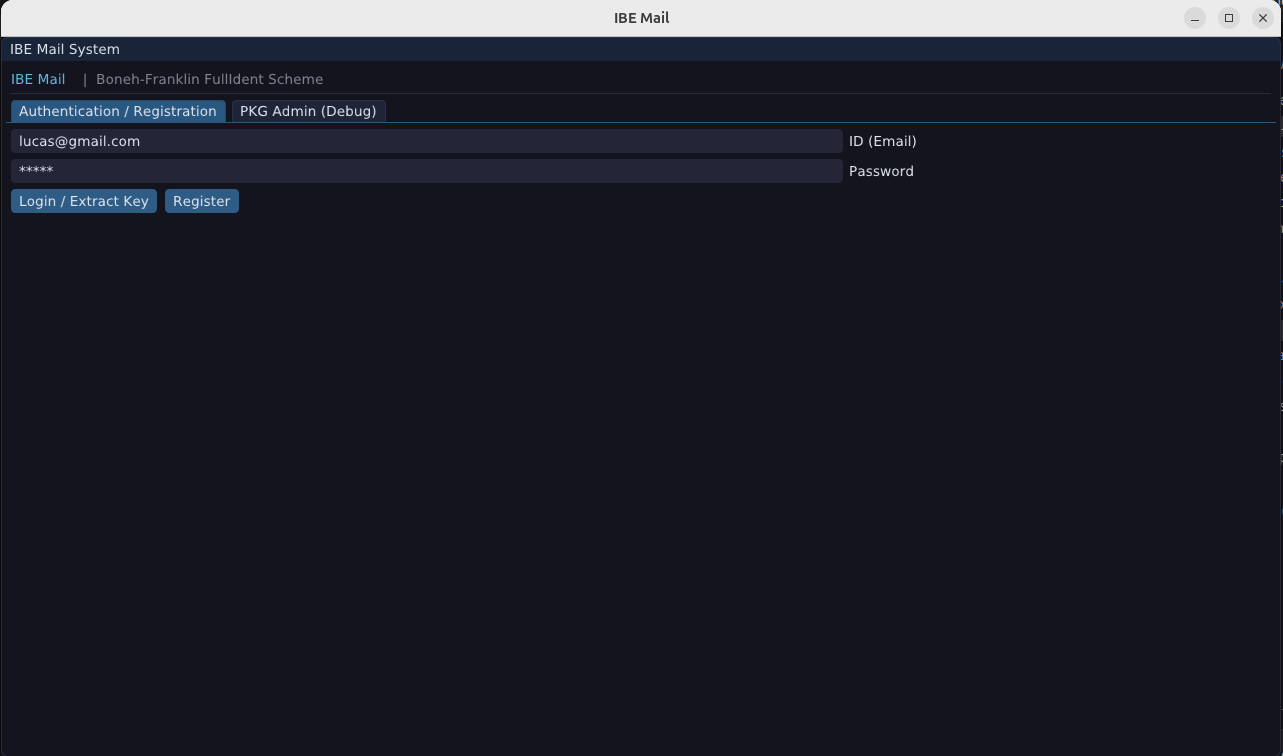
\includegraphics[width=0.9\textwidth]{images/1_registro.png}
    \caption{Tela de autenticação e solicitação de registro de identidade.}
    \label{fig:registro}
\end{figure}

Após o registro, a solicitação fica pendente no painel do administrador (Figura \ref{fig:pkg_pending}). O administrador do PKG, detentor do segredo mestre (\textit{Master Secret}), é responsável por aprovar a identidade do usuário. Ao clicar em \textit{Approve} (Figura \ref{fig:pkg_approved}), a chave privada do usuário é matematicamente derivada sobre a curva elíptica supersingular e armazenada em disco.

\begin{figure}[htb]
    \centering
    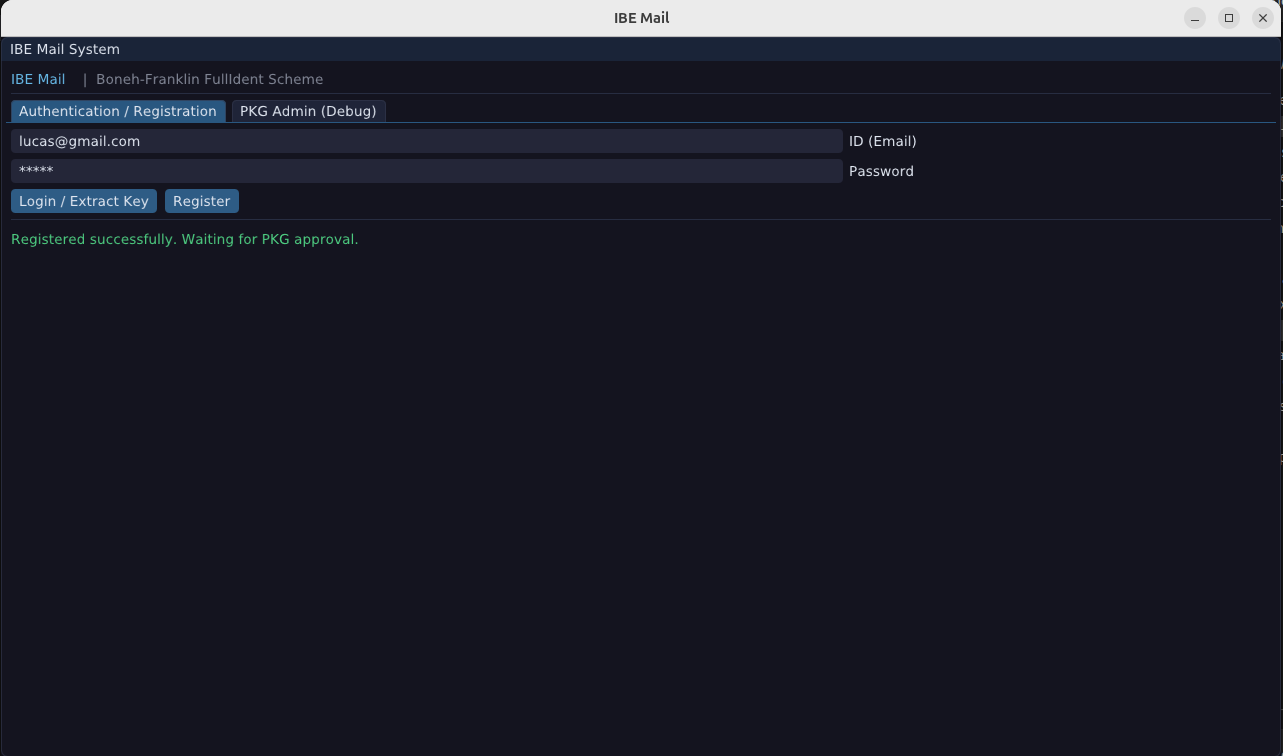
\includegraphics[width=0.9\textwidth]{images/2_pkg_pending.png}
    \caption{Solicitações pendentes.}
    \label{fig:pkg_pending}
\end{figure}

\begin{figure}[htb]
    \centering
    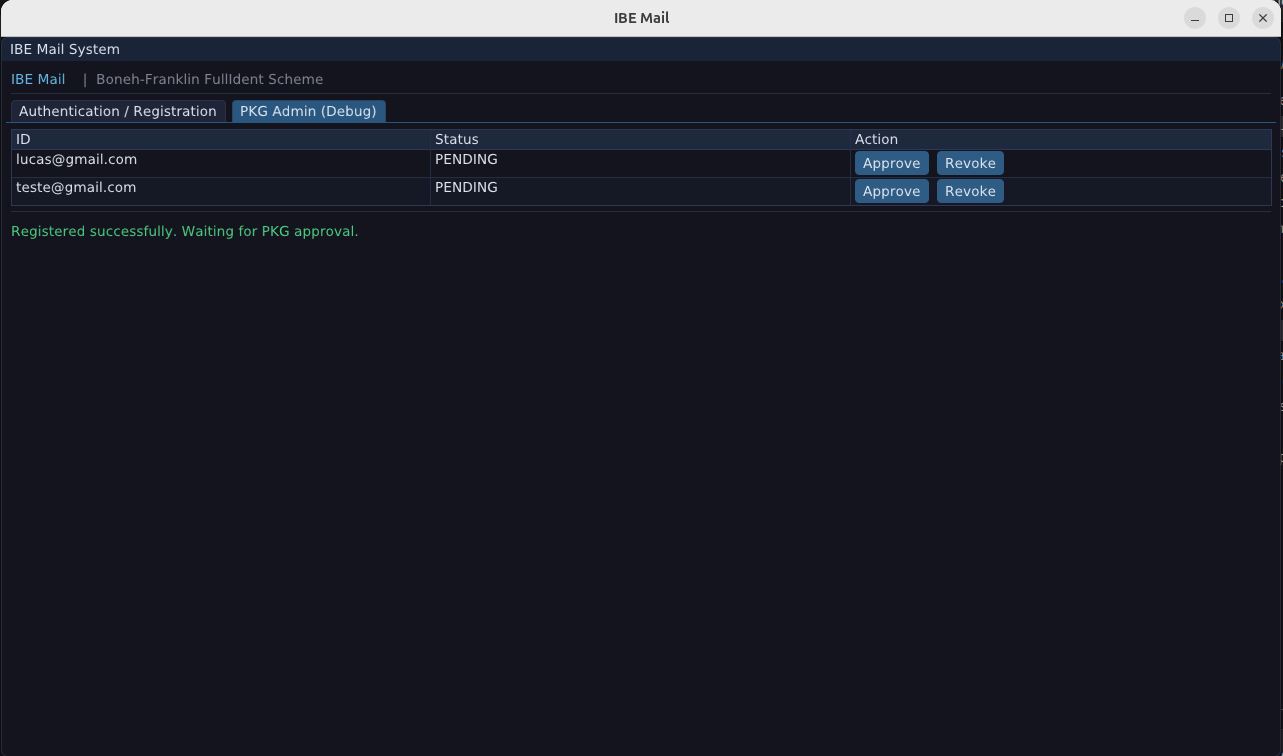
\includegraphics[width=0.9\textwidth]{images/3_pkg_approved.png}
    \caption{Aprovação de usuários.}
    \label{fig:pkg_approved}
\end{figure}

Com a aprovação, o usuário pode fazer o \textit{login} normalmente (Figura \ref{fig:auth_success}), obtendo acesso instantâneo ao uso de sua chave privada para a decifragem de mensagens.

\begin{figure}[htb]
    \centering
    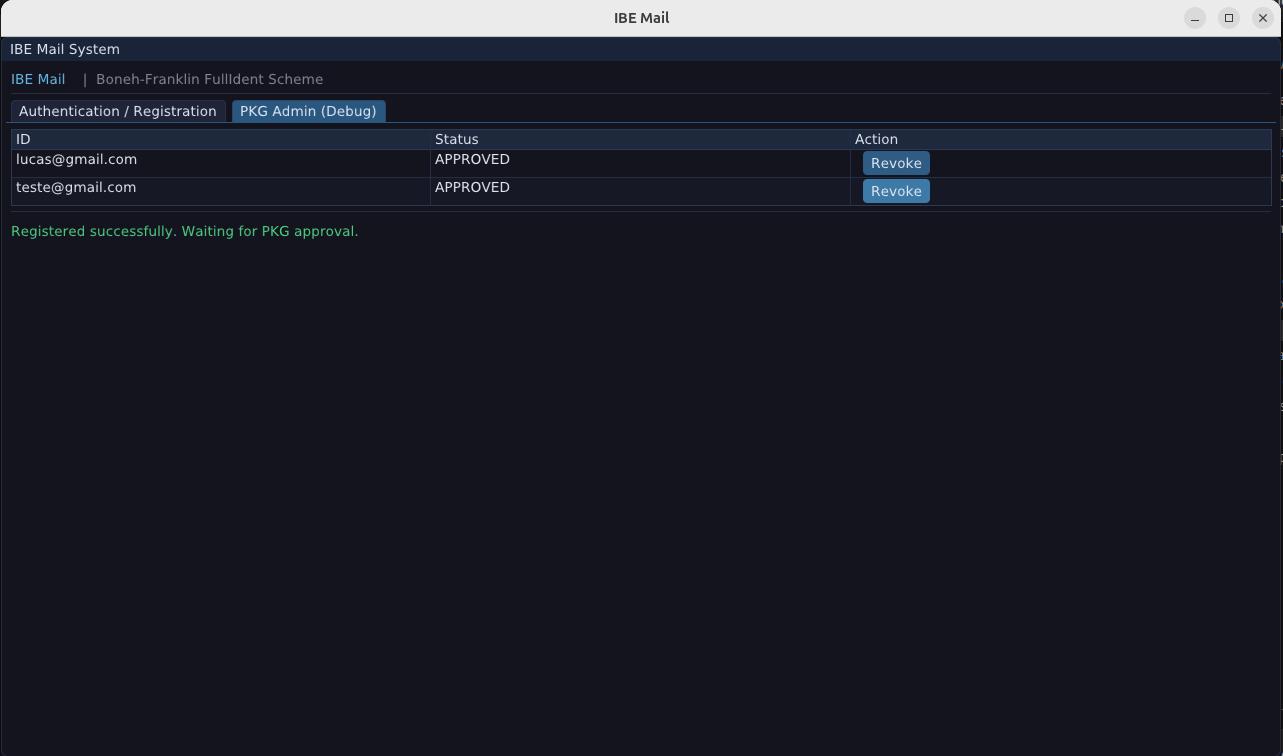
\includegraphics[width=0.9\textwidth]{images/4_auth_success.png}
    \caption{Usuário autenticado com sucesso e pronto para operar.}
    \label{fig:auth_success}
\end{figure}

\section{Troca de Mensagens}

Com usuários registrados no sistema, é possível demonstrar o roteamento e a decifragem de mensagens. A Figura \ref{fig:compose} mostra a formulação de um novo e-mail cifrado enviado de uma identidade para outra.

\begin{figure}[htb]
    \centering
    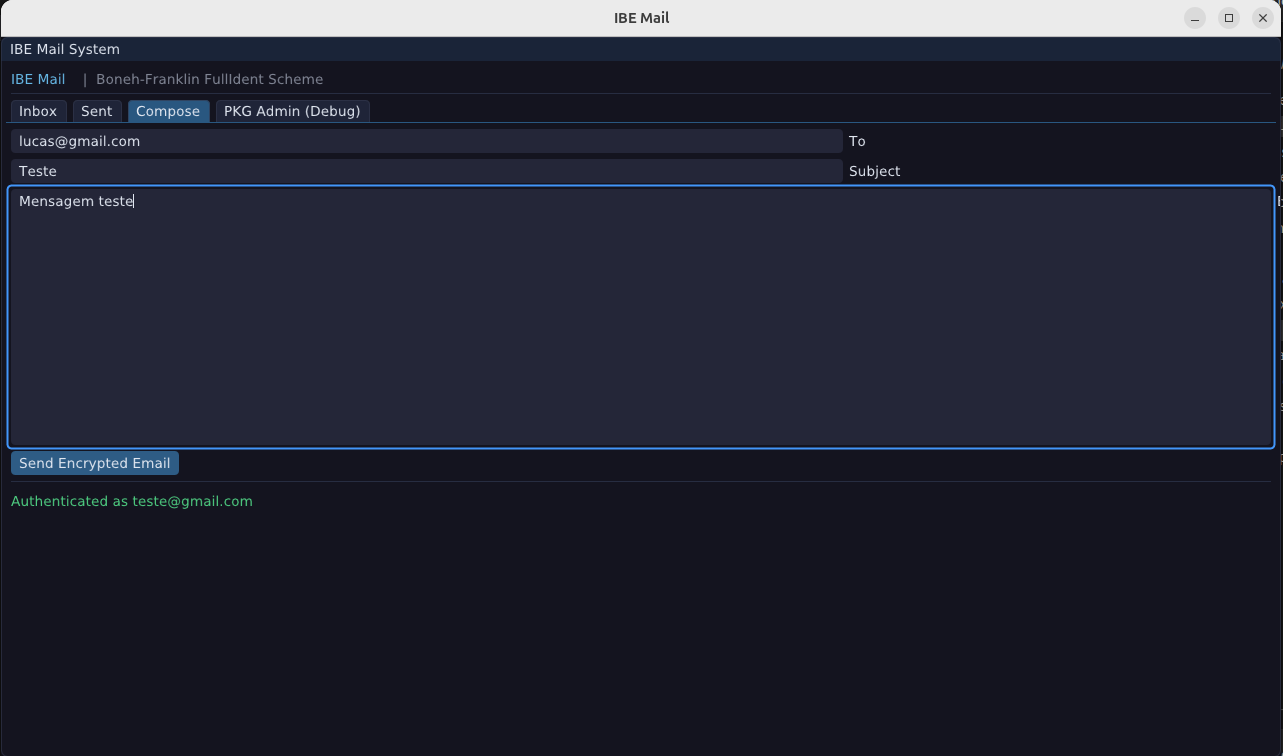
\includegraphics[width=0.9\textwidth]{images/5_compose.png}
    \caption{Interface de envio de mensagens cifradas.}
    \label{fig:compose}
\end{figure}

O remetente, após enviar o texto, pode observar na aba \textit{Sent} (Figura \ref{fig:sent}) os e-mails emitidos. O programa exibe o conteúdo do arquivo físico \texttt{.ibemail} gerado. É importante notar que o rementente não pode ler a mensagem que ele mesmo enviou, dado que o texto foi cifrado para a chave pública do destinatário.

\begin{figure}[htb]
    \centering
    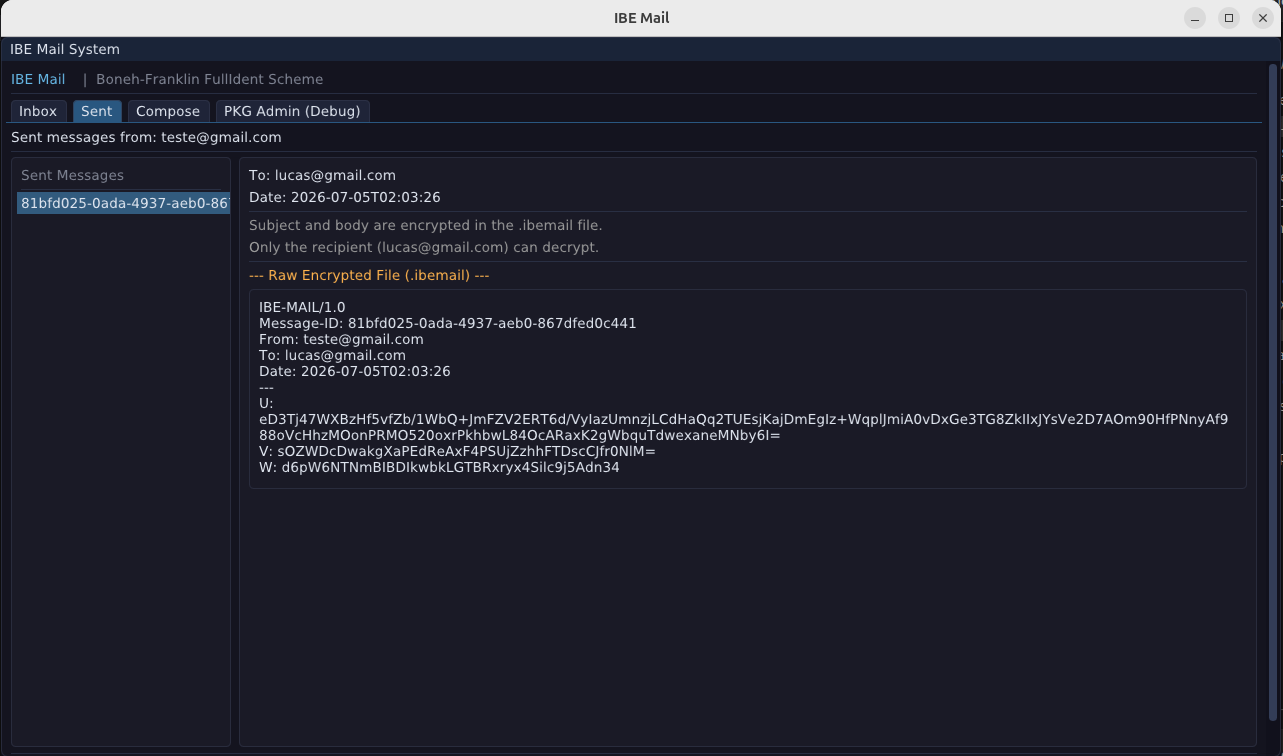
\includegraphics[width=0.9\textwidth]{images/6_sent.png}
    \caption{Aba de enviados exibindo os blocos de texto cifrado em Base64.}
    \label{fig:sent}
\end{figure}

Ao abrir a caixa de entrada (\textit{Inbox}) do destinatário \texttt{lucas@gmail.com}, o algoritmo \textit{Decrypt} extrai e reverte os blocos de informação utilizando a chave privada gerada na primeira etapa. A mensagem é decifrada de forma legível e perfeitamente íntegra (Figura \ref{fig:inbox}).

\begin{figure}[htb]
    \centering
    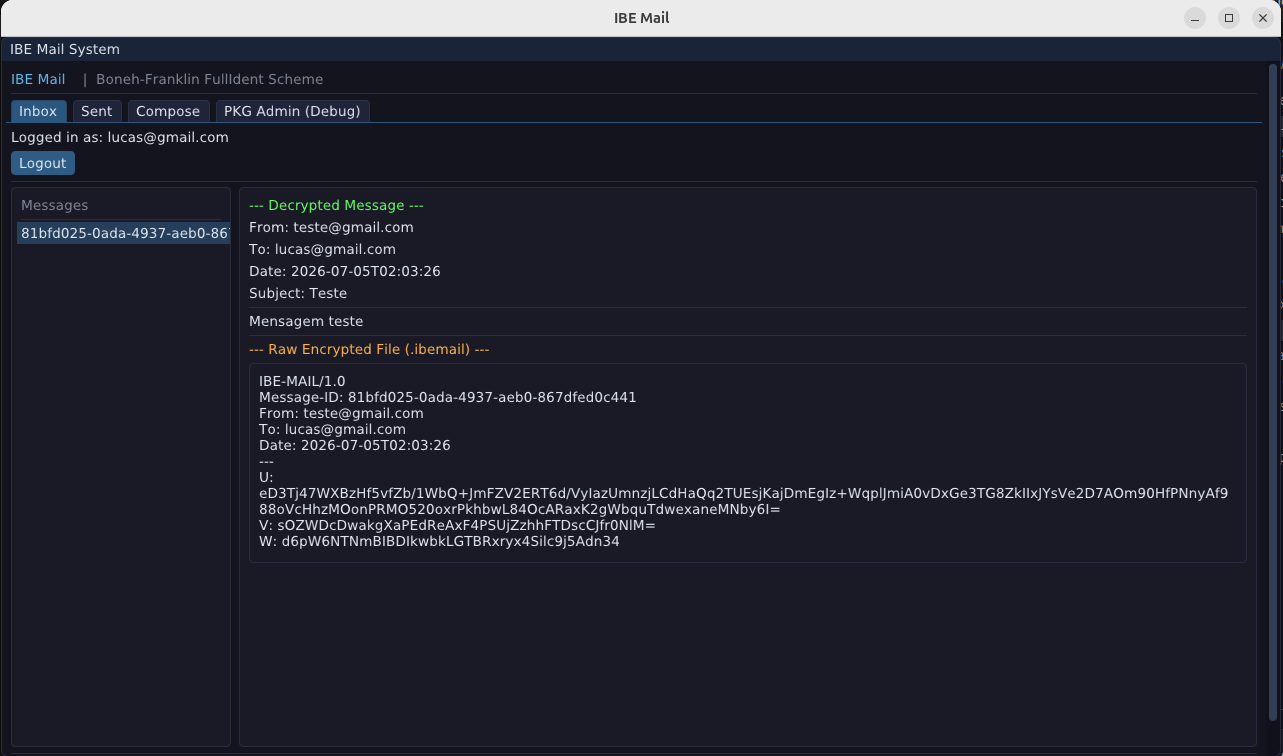
\includegraphics[width=0.9\textwidth]{images/7_inbox.png}
    \caption{Mensagem decifrada e lida com sucesso pelo destinatário.}
    \label{fig:inbox}
\end{figure}

\section{Segurança IND-ID-CCA2}

A implementação utiliza a transformação de Fujisaki-Okamoto (FO) para garantir que mensagens alteradas sejam ativamente rejeitadas no momento da decifragem, inviabilizando ataques de falsificação de texto cifrado.

Para provar esta propriedade na prática, o arquivo original de uma mensagem foi deliberadamente alterado via editor de código (Figura \ref{fig:file_alteration}), modificando-se um caractere do cifrotexto (bloco $U$).

\begin{figure}[htb]
    \centering
    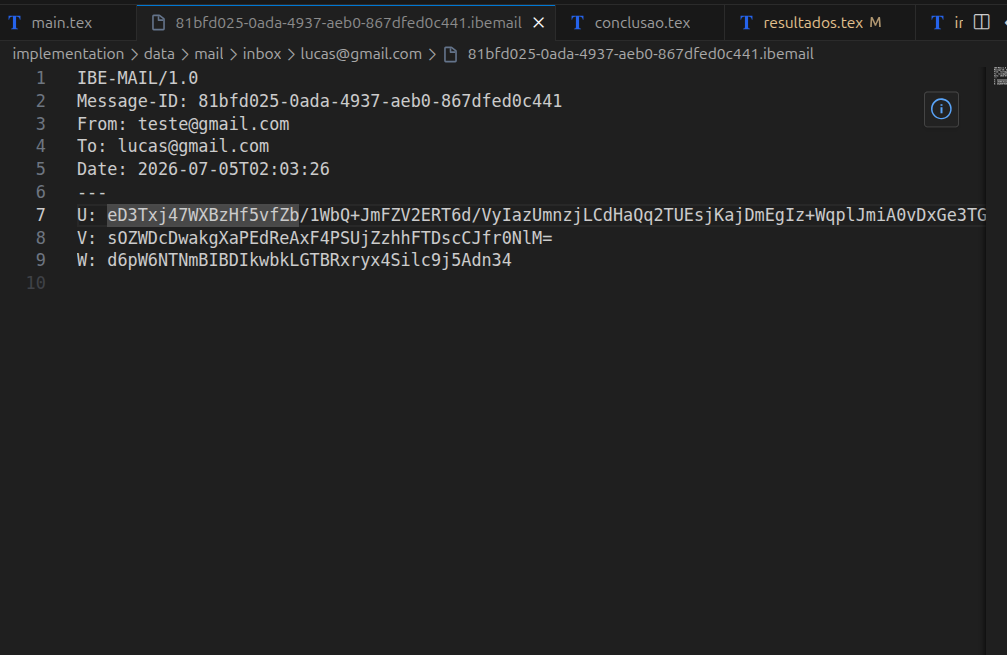
\includegraphics[width=0.9\textwidth]{images/8_file_alteration.png}
    \caption{Alteração maliciosa injetada no arquivo \texttt{.ibemail} utilizando um editor.}
    \label{fig:file_alteration}
\end{figure}

Ao retornar para a interface do programa e tentar ler a mensagem adulterada, a verificação de consistência hash de Fujisaki-Okamoto ($U = r \cdot P$) falha. O sistema detecta a violação, lança um erro e impede a leitura (Figura \ref{fig:cca2_rejection}), garantindo a resiliência (CCA2) do protocolo IBE contra adulterações ativas.

\begin{figure}[htb]
    \centering
    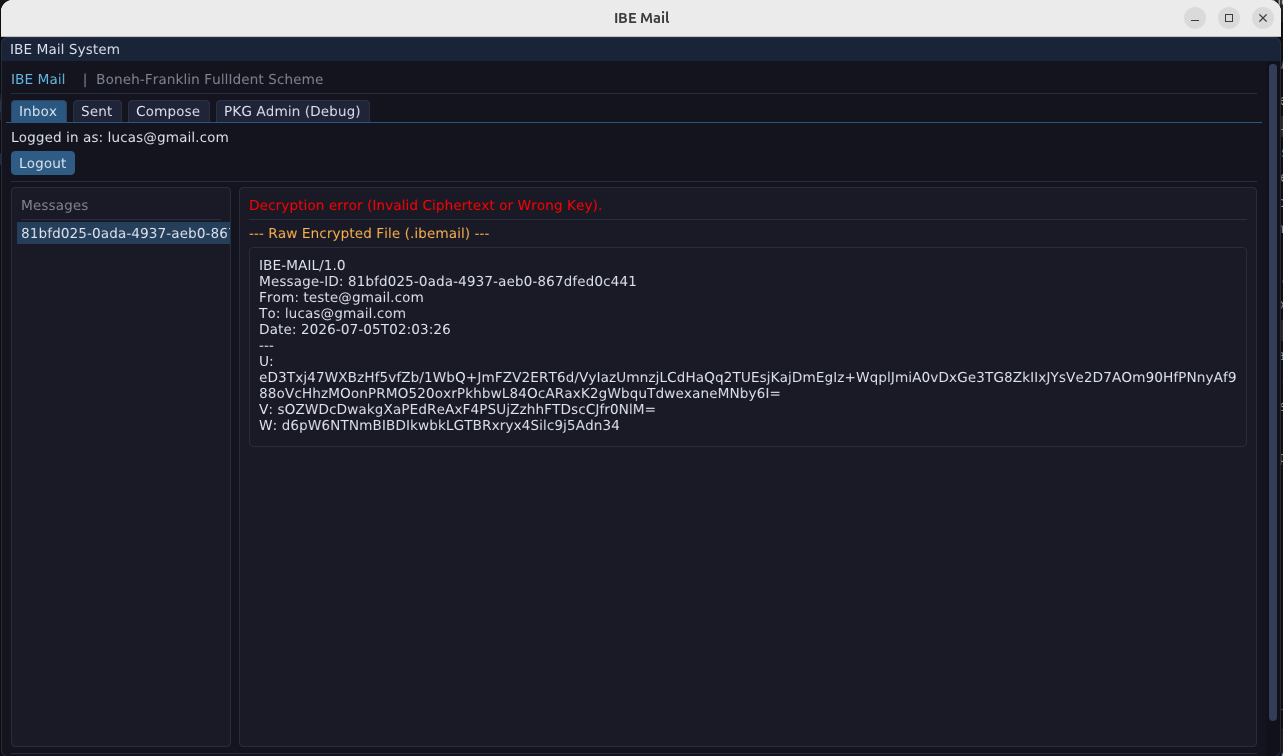
\includegraphics[width=0.9\textwidth]{images/9_cca2_rejection.png}
    \caption{Rejeição imediata do cifrotexto devido a quebra de integridade (CCA2).}
    \label{fig:cca2_rejection}
\end{figure}

\section{Identidades Temporais (Cifragem para o Futuro)}

Uma das características mais marcantes da Criptografia Baseada em Identidade é a capacidade de cifrar dados sigilosos para chaves que sequer foram geradas pelo PKG.

No teste final, uma mensagem foi endereçada à identidade \texttt{teste2@gmail.com|2026-06} (Figura \ref{fig:time_sent}), demonstrando o particionamento de uma identidade no tempo (útil para processos de revogação periódica natural). O e-mail foi cifrado utilizando essa estrutura (\textit{string}) literal como chave pública matemática, sem que a chave privada real existisse naquele momento.

\begin{figure}[htb]
    \centering
    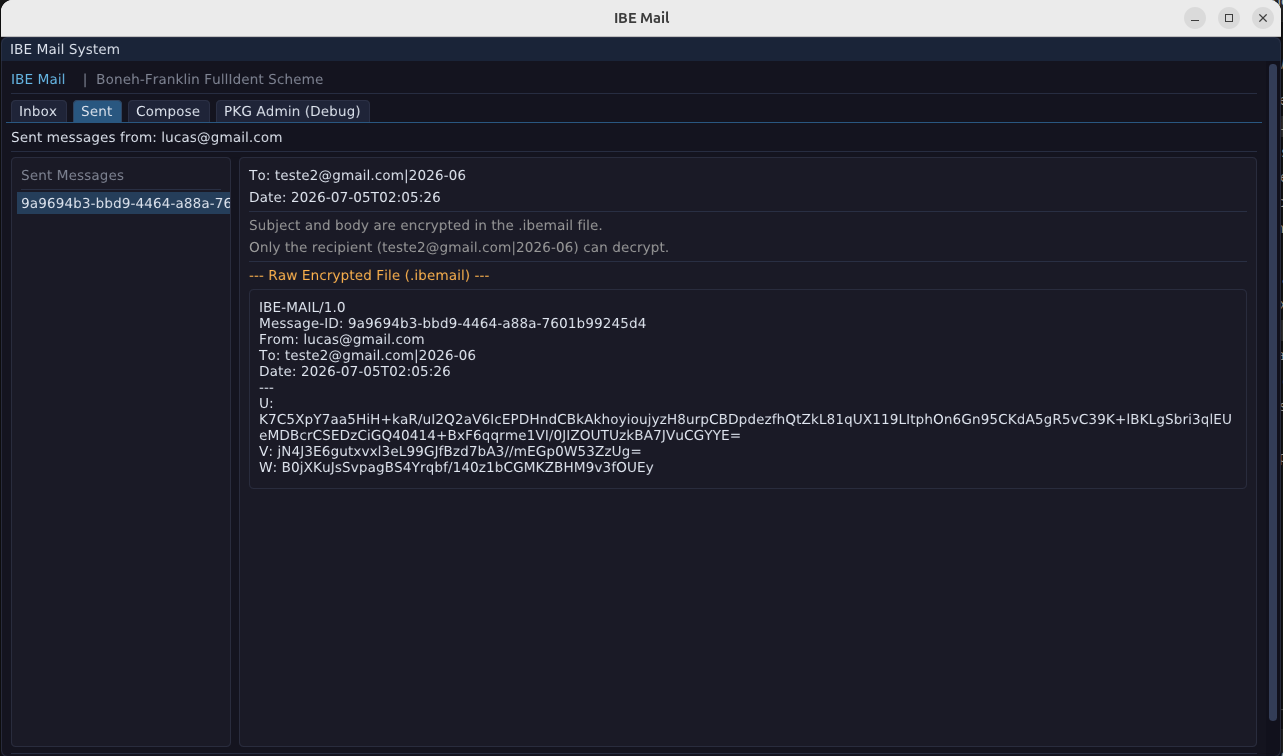
\includegraphics[width=0.9\textwidth]{images/10_time_sent.png}
    \caption{Envio de e-mail assíncrono para uma identidade contendo partição de data.}
    \label{fig:time_sent}
\end{figure}

Posteriormente, a identidade exata particionada (\texttt{teste2@gmail.com|2026-06}) foi registrada no sistema e aprovada no PKG. Ao logar com essa credencial temporal, o usuário conseguiu recuperar sua chave privada retroativamente e ler as mensagens que lhe foram destinadas, comprovando na prática o dinamismo e o roteamento exato da abordagem de Boneh-Franklin (Figura \ref{fig:time_inbox}).

\begin{figure}[htb]
    \centering
    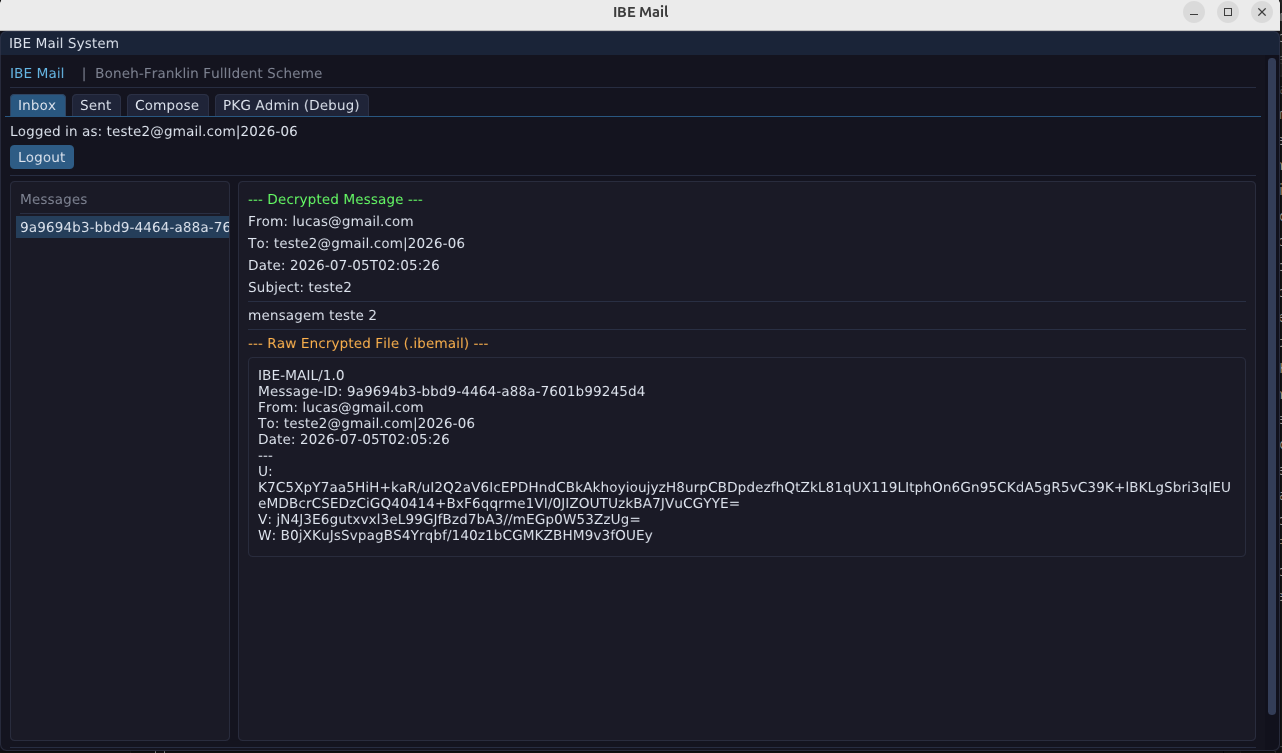
\includegraphics[width=0.9\textwidth]{images/11_time_inbox.png}
    \caption{Usuário logado sob a identidade de tempo específica para recuperar as mensagens.}
    \label{fig:time_inbox}
\end{figure}

    \chapter{Conclusão}
\label{cap:conclusao}

O desenvolvimento deste trabalho confirmou de forma prática todas as proposições da literatura sobre Criptografia Baseada em Identidade do tipo Boneh-Franklin. 
Ao integrar a matemática acadêmica de bilineariedade da PBC com as engenharias de software de aplicações visuais de usuário final (Dear ImGui), foi possível tangibilizar as vantagens do IBE frente às restrições do PKI tradicional, atingindo 100\% dos requisitos planejados.


    \postextual
    \setlength\beforechapskip{0pt}
    \setlength\midchapskip{15pt}
    \setlength\afterchapskip{15pt}

    \begingroup
        \setlength\bibitemsep{\baselineskip}
        \nocite{claude2026ai}
        \nocite{gemini2026ai}
        \printbibliography[title=REFERÊNCIAS]
    \endgroup

\end{document}
